\documentclass[a4paper,14pt]{extreport}
\usepackage[utf8]{inputenc} % Set Encoding
\usepackage[T1,T2A]{fontenc}
\usepackage{fontspec} % Using custom fonts (requires -xelatex flag)
\usepackage[russian,english,ukrainian]{babel} % Using languages
\usepackage{geometry} % Set margins
\usepackage[raggedright]{titlesec} % For section modification
\usepackage{indentfirst} % Inserts indents in paragraphs
\usepackage{minted} % For code listing
\usepackage{graphicx} % For image insertions
\usepackage{float} % For positioning
\usepackage[section]{placeins}
\usepackage{fancyhdr}
\usepackage{caption}
\usepackage{enumitem} % List indents
\usepackage{chngcntr}
\usepackage[english,russian,ukrainian]{babel}
\usepackage[nottoc]{tocbibind}
\usepackage{color}
\usepackage{xpatch}
\definecolor{spot}{rgb}{0,0,0}
\usepackage[colorlinks,allcolors=spot,bookmarksopen=true,pdfstartview=FitH]{hyperref}

\counterwithout{section}{chapter}

\pagestyle{fancy}

\fancyhf{}
\fancyhead[R]{\thepage}
\renewcommand{\headrulewidth}{0pt}
\fancyheadoffset{0mm}
\fancyfootoffset{0mm}
\renewcommand{\headrulewidth}{0pt}
\renewcommand{\footrulewidth}{0pt}
\setlength{\headheight}{17.0pt}

\fancypagestyle{plain}{
    \fancyhf{}
    \rhead{\thepage}}


\pagenumbering{gobble}

\usemintedstyle{bw}

\geometry{
  a4paper,
  left=30mm,
  right=20mm,
  top=20mm,
  bottom=20mm
}

\DeclareCaptionLabelFormat{gostfigure}{Рисунок #2}
\DeclareCaptionLabelFormat{gosttable}{Таблиця #2}
\DeclareCaptionLabelSeparator{gost}{~---~}
\captionsetup{labelsep=gost}
\captionsetup[figure]{labelformat=gostfigure, justification=centering,
labelsep=gost}
\captionsetup[table]{labelformat=gosttable, labelsep=gost}

\setlength\parindent{2.5em}
\renewcommand{\baselinestretch}{2.0}
\linespread{1.3} % Set default line spacing

\setmainfont{Liberation Serif} % Set default font on Linux

\titleformat{\section}
{\normalfont}{\thesection}{1em}{}

\titleformat{\subsection}
{\normalfont}{\thesubsection}{1em}{}

\titleformat{\subsubsection}
{\normalfont}{\thesubsubsection}{1em}{}

\titleformat{\chapter}[block]
    {\filcenter\bfseries}
    {\thechapter}
    {1em}
    {\MakeUppercase}{}

\renewcommand{\headrulewidth}{0pt}

\titlespacing{\chapter}{0pt}{-30pt}{2em}
\titlespacing\section{0cm}{2em}{1ex}
\titlespacing\subsection{0cm}{1ex}{1ex}

\newcommand\chap[1]{%
  \chapter*{#1}%
  \addcontentsline{toc}{chapter}{\uppercase{#1}}}

\graphicspath{{./pics}}

\setlist[enumerate]{leftmargin=4em}

\begin{document}
\begin{titlepage}
	\centering
    Міністерство освіти і науки України
    
    Харківський національний університет радіоелектроніки
    \vspace{1cm}

    Факультет комп'ютерних наук
    \vspace{1cm}

    Кафедра штучного інтелекту

    \vspace{2cm}
    \uppercase{Реферат}
    \vspace{1cm}

    на тему <<Бот Dvango>>
    \vspace{1cm}

    з дисципліни <<Системи інтелектуальної обробки природно-мовної інформації>>

    \begin{flushleft}
    \vspace{4cm}
    \begin{minipage}[t]{8cm}
        Виконали ст. гр. ІТШІ-18-1:

        Соколенко Дмитро Олександрович

        Апраксін Антон Романович
    \end{minipage}
    \hfill
    \begin{minipage}[t]{6cm}
        Прийняв:\\
        проф. каф. ШІ Рябова Н. В.\\
        з оцінкою ``\rule{2cm}{0.15mm}''\\
        ``\rule{0.7cm}{0.15mm}''\rule{2cm}{0.15mm}20\rule{0.7cm}{0.15mm}р
    \end{minipage}
    \end{flushleft}
	\vfill

	{Харків \the\year{}}
\end{titlepage}
\pagenumbering{arabic}
\setcounter{page}{3}

\chap{Реферат}


\newpage
\tableofcontents
\newpage




\chap{Вступ}


\chap{Основна частина}
\section{Аналіз предметної галузі}
\subsection{Штучні нейронні мережі}
Штучна нейронна мережа побудована навколо біологічної метафори.
Будова первинної зорової кори відносно добре відома,
і вчені виграли Нобелівську премію з фізіології за відкриття в
1962 р. організації нейронів у перших кортикальних
шарах \cite{cortex-stuff}. Таким чином, в надзвичайно
спрощеному вигляді
мозку нейрони організовані шарами, кожен нейрон отримує
інформацію з попереднього шару, виконує дуже просте
обчислення і передає свій результат нейронам наступного
шару. Однак слід пам’ятати, що це лише метафора та джерело
натхнення: біологічні мережі мають набагато складніші
зв’язки, а математичні рівняння, що керують ними, також
є більш складними \cite{cortex-equations}.



\subsection{Рекурентні нейронні мережі}

\subsection{Механізм уваги}
Увага до певної міри мотивована тим, як ми приділяємо зорову увагу
різним регіонам зображення або співвідносимо слова в одному реченні.

Зорова увага людини дозволяє зосередитись на певному регіоні з
``високою роздільною здатністю'', одночасно сприймаючи навколишнє
зображення в ``низькій роздільній здатності'', а потім відрегувати
фокусну точку або зробити відповідний висновок.
Враховуючи невеликий фрагмент зображення, пікселі в решті надають підказки, що
там відображається. Ми очікуємо побачити загострене вухо в жовтій коробці,
тому що ми бачили ніс собаки, ще одне загострене вухо праворуч і очі
Шіби (речі в червоних квадратах) (Рис. \ref{fig:shiba}). Однак светр та ковдра внизу були
б не такими корисними, як ті собачі риси.

\begin{figure}[H]
    \centering
    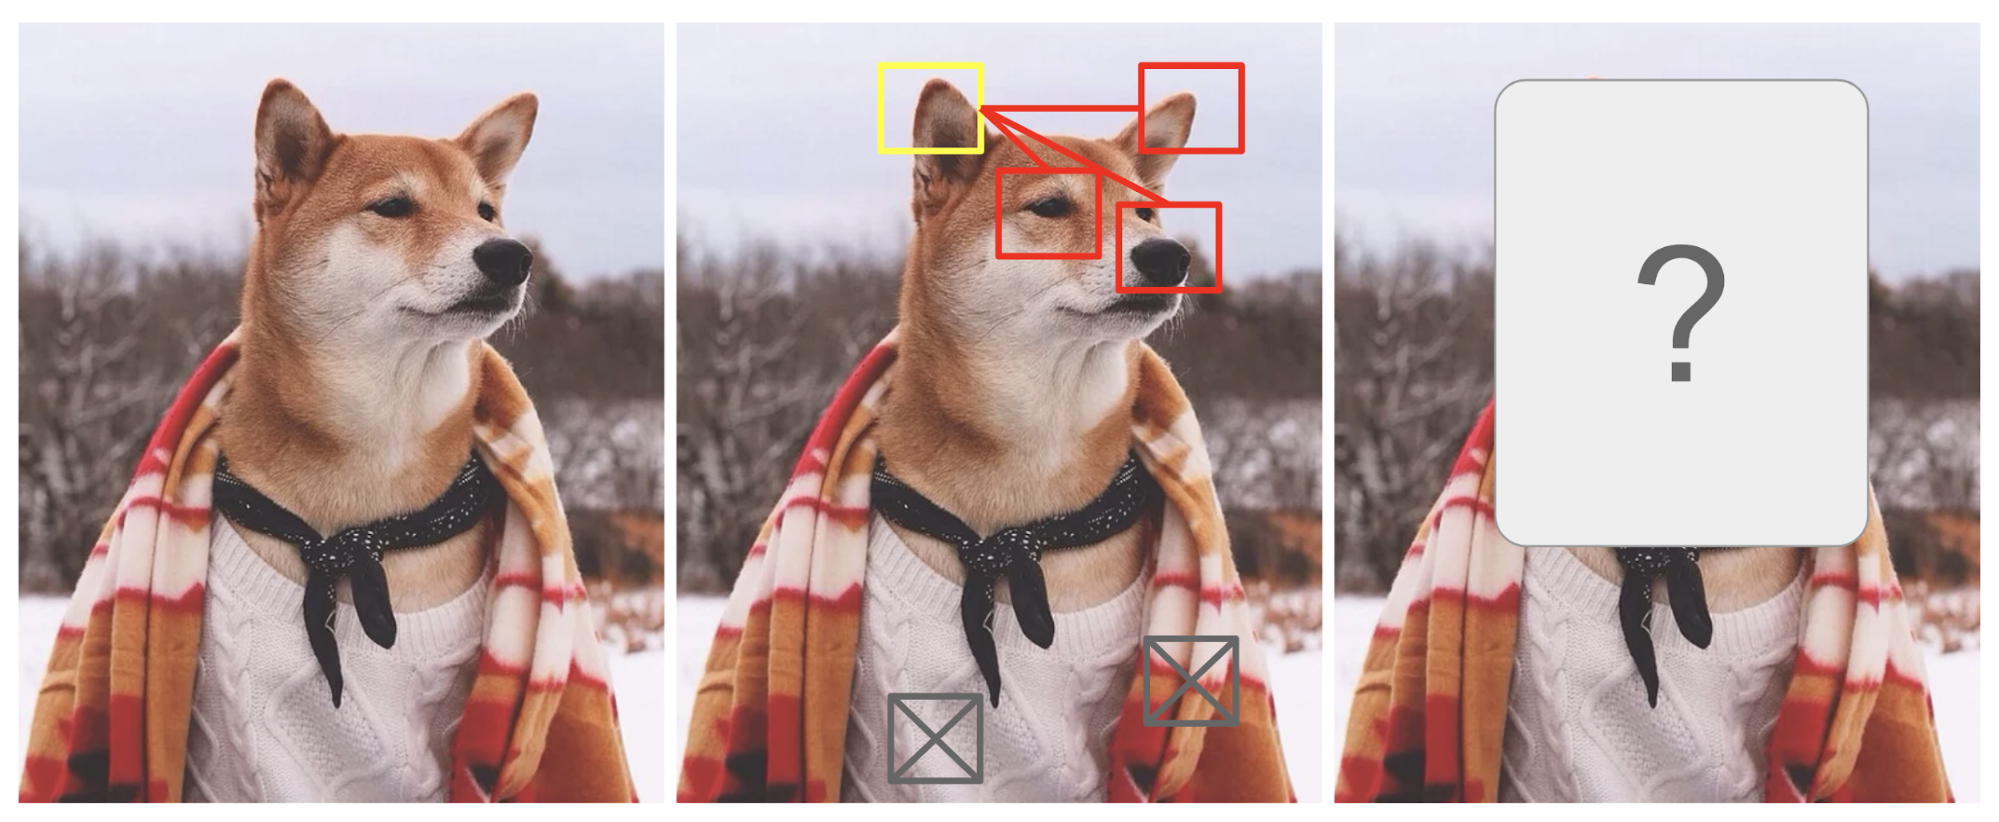
\includegraphics[width=0.75\textwidth]{shiba-example-attention.png}
    \caption{Шіба-іну в одязі}
    \label{fig:shiba}
\end{figure}

Подібним чином ми можемо пояснити зв'язок між словами в одному реченні
або близькому контексті. Коли ми бачимо ``їсти'', ми сподіваємось дуже
скоро зустріти слово, що означає вид їжи.

\begin{figure}[H]
    \centering
    
\includegraphics[width=0.75\textwidth]{sentence-example-attention.png}
    \caption{Одне слово ``поділяє увагу'' іншим словам по-різному}
    \label{fig:attend-example}
\end{figure}

Увагу при глибокому навчанні можна широко трактувати як вектор вагових
коефіцієнтів: для того, щоб передбачити або зробити висновок про один елемент,
наприклад, піксель на зображенні або слово в реченні, ми оцінюємо,
використовуючи вектор уваги, наскільки сильно він співвідноситься з іншими
елементами,
і приймає суму їх значень, зважену вектором уваги, як наближення
цілі \cite{attention}.

Архітектури, засновані на трансформаторах, які в основному
використовуються для моделювання завдань на розуміння мови,
уникають використання рекурентності у нейронних мережах і замість
цього цілком довіряють механізмам самоуваги для побудови
глобальних залежностей між входами та виходами.

\section{Теоретичні дослідження}


\section{Експериментальні дослідження}


\newpage
\renewcommand\bibname{ПЕРЕЛІК ДЖЕРЕЛ ПОСИЛАННЯ}
\begin{thebibliography}{9}
    \bibitem{latex:friends}
    What are TeX and its friends? [Електронний ресурс] – Режим доступу до ресурсу: https://www.ctan.org/tex.

    \bibitem{latex:oss-devs-latex}
    Gaudeul A. Do Open Source Developers Respond to Competition? The LATEX Case Study / Alex Gaudeul. // Review of Network Economics. – 2007.

    \bibitem{webhooks:define}
    Webhooks [Електронний ресурс]. – 2019. – Режим доступу до ресурсу: https://developer.atlassian.com/server/jira/platform/webhooks/.

    \bibitem{webhooks:good}
    Lindsay J. Web hooks to revolutionize the web [Електронний ресурс] / Jeff Lindsay. – 2007. – Режим доступу до ресурсу: https://web.archive.org/web/20180630220036/http://progrium.com/blog/2007/05/03/web-hooks-to-revolutionize-the-web/.
    
    \bibitem{transformers:repo}
    State-of-the-art Natural Language Processing for Jax, PyTorch and TensorFlow [Електронний ресурс] – Режим доступу до ресурсу: https://github.com/huggingface/transformers.

    \bibitem{flashtext:arxiv}
    Replace or Retrieve Keywords In Documents at Scale [Електронний ресурс]. – 2017. – Режим доступу до ресурсу: https://arxiv.org/abs/1711.00046.

    \bibitem{flashtext:repo}
    FlashText module [Електронний ресурс] – Режим доступу до ресурсу: https://github.com/vi3k6i5/flashtext.

    \bibitem{ahocorasik:wiki}
    Aho–Corasick algorithm [Електронний ресурс] – Режим доступу до ресурсу: https://en.wikipedia.org/wiki/Aho%E2%80%93Corasick_algorithm.

    \bibitem{attention}
    Weng L. Attention? Attention! [Електронний ресурс] / Lilian Weng // lilianweng.github.io/lil-log. – 2018. – Режим доступу до ресурсу: http://lilianweng.github.io/lil-log/2018/06/24/attention-attention.html.

    \bibitem{cortex-stuff}
    Hubel D. Receptive fields, binocular interaction and functional architecture in the cat’s visual cortex / D. Hubel, T. Wiesel. // The Journal of physiology. – 1962. – С. 106–154.

    \bibitem{cortex-equations}
    Hodgkin A. quantitative description of membrane current and its application to conduction and excitation in nerve / A. Hodgkin, A. Huxley. // The Journal of physiology. – 1952. – С. 500–544.

    \bibitem{rozenblatt}
    Rosenblatt F. The perceptron, a perceiving and recognizing automaton Project Para / Frank Rosenblatt. // Cornell Aeronautical Laboratory. – 1957.

    \bibitem{nn:peyre}
    Peyré G. Mathematics of Neural Networks [Електронний ресурс] / Gabriel Peyré – Режим доступу до ресурсу: https://mathematical-tours.github.io/book-basics-sources/neural-networks-en/NeuralNetworksEN.pdf.

    \bibitem{nn:backpropagation}
    Rumelhart D. Learning representations by back-propagating errors / D. Rumelhart, G. Hinton, R. Williams. // nature. – 1986. – С. 533–536.

    \bibitem{gradient-descend}
    Ruder S. An overview of gradient descent optimization algorithms / Sebastian Ruder. // arXiv preprint arXiv:1609.04747. – 2016.

    \bibitem{nn:multilayer-perceptrons}
    Grosse R. Lecture 5: Multilayer Perceptrons [Електронний ресурс] / Roger Grosse – Режим доступу до ресурсу: https://www.cs.toronto.edu/~mren/teach/csc411\_19s/lec/lec10\_notes1.pdf.
\end{thebibliography}

\newpage
\chap{Додаток 1}
% \centerline{\uppercase{\bf{Програмна реалізація}}}
%     \inputminted[breaklines,linenos=true]{python}{../../src/app.py}

% \chap{Додаток 2}
% \centerline{\uppercase{\bf{Результати роботи}}}
%     \begin{figure}[H]
%         \centering
%         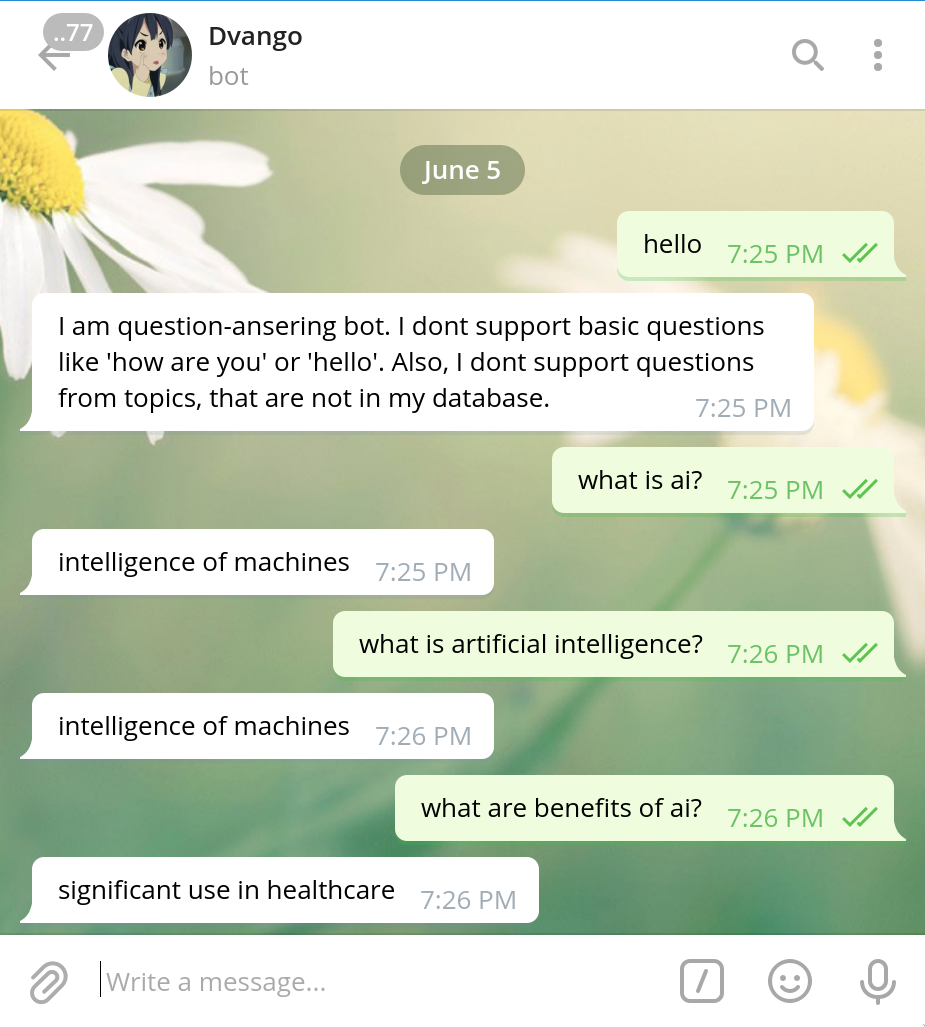
\includegraphics[width=0.75\textwidth]{f1.png}
%     \end{figure}
    
%     \begin{figure}[H]
%         \centering
%         
\includegraphics[width=0.75\textwidth]{f2.png}
%     \end{figure}

%     \begin{figure}[H]
%         \centering
%         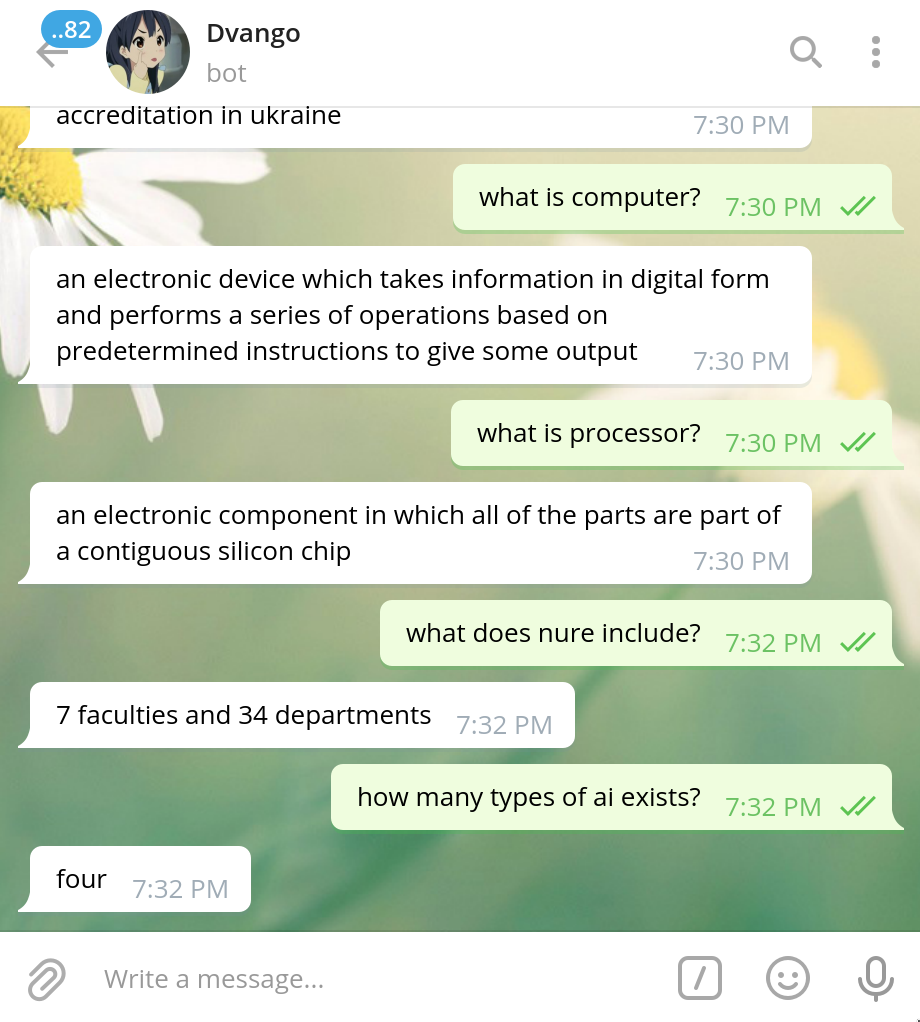
\includegraphics[width=0.75\textwidth]{f3.png}
%     \end{figure}
\end{document}


% \begin{figure}[H]
%     \centering
%     \includegraphics[width=0.75\textwidth]{rplot_iris.png}
%     \caption{Графік дерева вибірки Iris з дискретизацією через IG}
%     \label{fig:plot3}
% \end{figure}

% \begin{table}[H]
%     \centering
%     \begin{tabular}{ |c|c|c|c| } 
%      \hline
%      Мова   & \multicolumn{3}{c|}{Метод та датасет} \\ \hline
%             & Iris Thr. & Iris IG & SUSY \\ \hline
%      Python & 0.9333    & 0.9333  & 0.6799 \\ \hline
%      R      & 0.9333    & 0.9777  & 0.6594 \\ 
%      \hline
%     \end{tabular}
%     \caption{Порівняння точності класифікації}
%     \label{tab:t1}
% \end{table}
% \inputminted[breaklines,linenos=true]{scilab}{repl235.txt}
